% =====================================================================
%  RidePool -- Level 1 Data Flow Diagram (Gane-Sarson notation)
%  Standalone TikZ figure. Compile with pdflatex/lualatex/xelatex.
%
%  To use it inside your report instead, copy everything between
%  "BEGIN FIGURE" and "END FIGURE" into your document and make sure the
%  preamble lines marked (*) are present in your own preamble.
% =====================================================================
\documentclass[border=4pt]{standalone}

\usepackage[T1]{fontenc}          % (*)
\usepackage{tikz}                 % (*)
\usetikzlibrary{arrows.meta}      % (*)
\usepackage{xcolor}               % (*)

% ---- (*) palette: taken from the RidePool design tokens -------------
\definecolor{riderblue}{HTML}{2563EB}
\definecolor{riderbg}{HTML}{EFF6FF}
\definecolor{inkdark}{HTML}{111827}
\definecolor{inkgrey}{HTML}{374151}
\definecolor{midgrey}{HTML}{6B7280}
\definecolor{slategrey}{HTML}{4B5563}
\definecolor{surfacegrey}{HTML}{F9FAFB}
\definecolor{hairline}{HTML}{D1D5DB}

% ---- (*) styles -----------------------------------------------------
\tikzset{
  proc/.style   ={rectangle, rounded corners=3pt, draw=riderblue, fill=riderbg,
                  line width=0.5pt, minimum width=4.70cm, minimum height=0.94cm,
                  align=center, inner sep=1pt, font=\scriptsize, text=inkdark},
  ent/.style    ={rectangle, draw=inkdark, fill=white, line width=0.6pt,
                  minimum width=2.20cm, minimum height=0.94cm, align=center,
                  inner sep=1pt, font=\scriptsize\bfseries, text=inkdark},
  extent/.style ={ent, minimum width=3.66cm},
  flow/.style   ={draw=inkgrey, line width=0.4pt,
                  {Stealth[length=1.5mm,width=1.1mm]}-{Stealth[length=1.5mm,width=1.1mm]}},
  sflow/.style  ={draw=midgrey, line width=0.4pt,
                  {Stealth[length=1.5mm,width=1.1mm]}-{Stealth[length=1.5mm,width=1.1mm]}},
  lbl/.style    ={midway, fill=white, inner sep=1pt, font=\tiny, text=slategrey},
}

% ---- (*) open-ended data store: #1 x, #2 y, #3 id, #4 line, #5 line --
\newcommand{\dstore}[5]{%
  \begin{scope}[shift={(#1,#2)}]
    \fill[surfacegrey] (-2.2,-0.395) rectangle (2.2,0.395);
    \draw[draw=midgrey, line width=0.5pt]
         (2.2,0.395) -- (-2.2,0.395) -- (-2.2,-0.395) -- (2.2,-0.395);
    \draw[draw=midgrey, line width=0.5pt] (-1.85,0.395) -- (-1.85,-0.395);
    \node[font=\scriptsize\bfseries, text=inkgrey] at (-2.025,0) {#3};
    \node[anchor=west, font=\tiny, text=inkdark] at (-1.78, 0.17) {#4};
    \node[anchor=west, font=\tiny, text=midgrey] at (-1.78,-0.17) {#5};
  \end{scope}%
}

\begin{document}
% ============================ BEGIN FIGURE ===========================
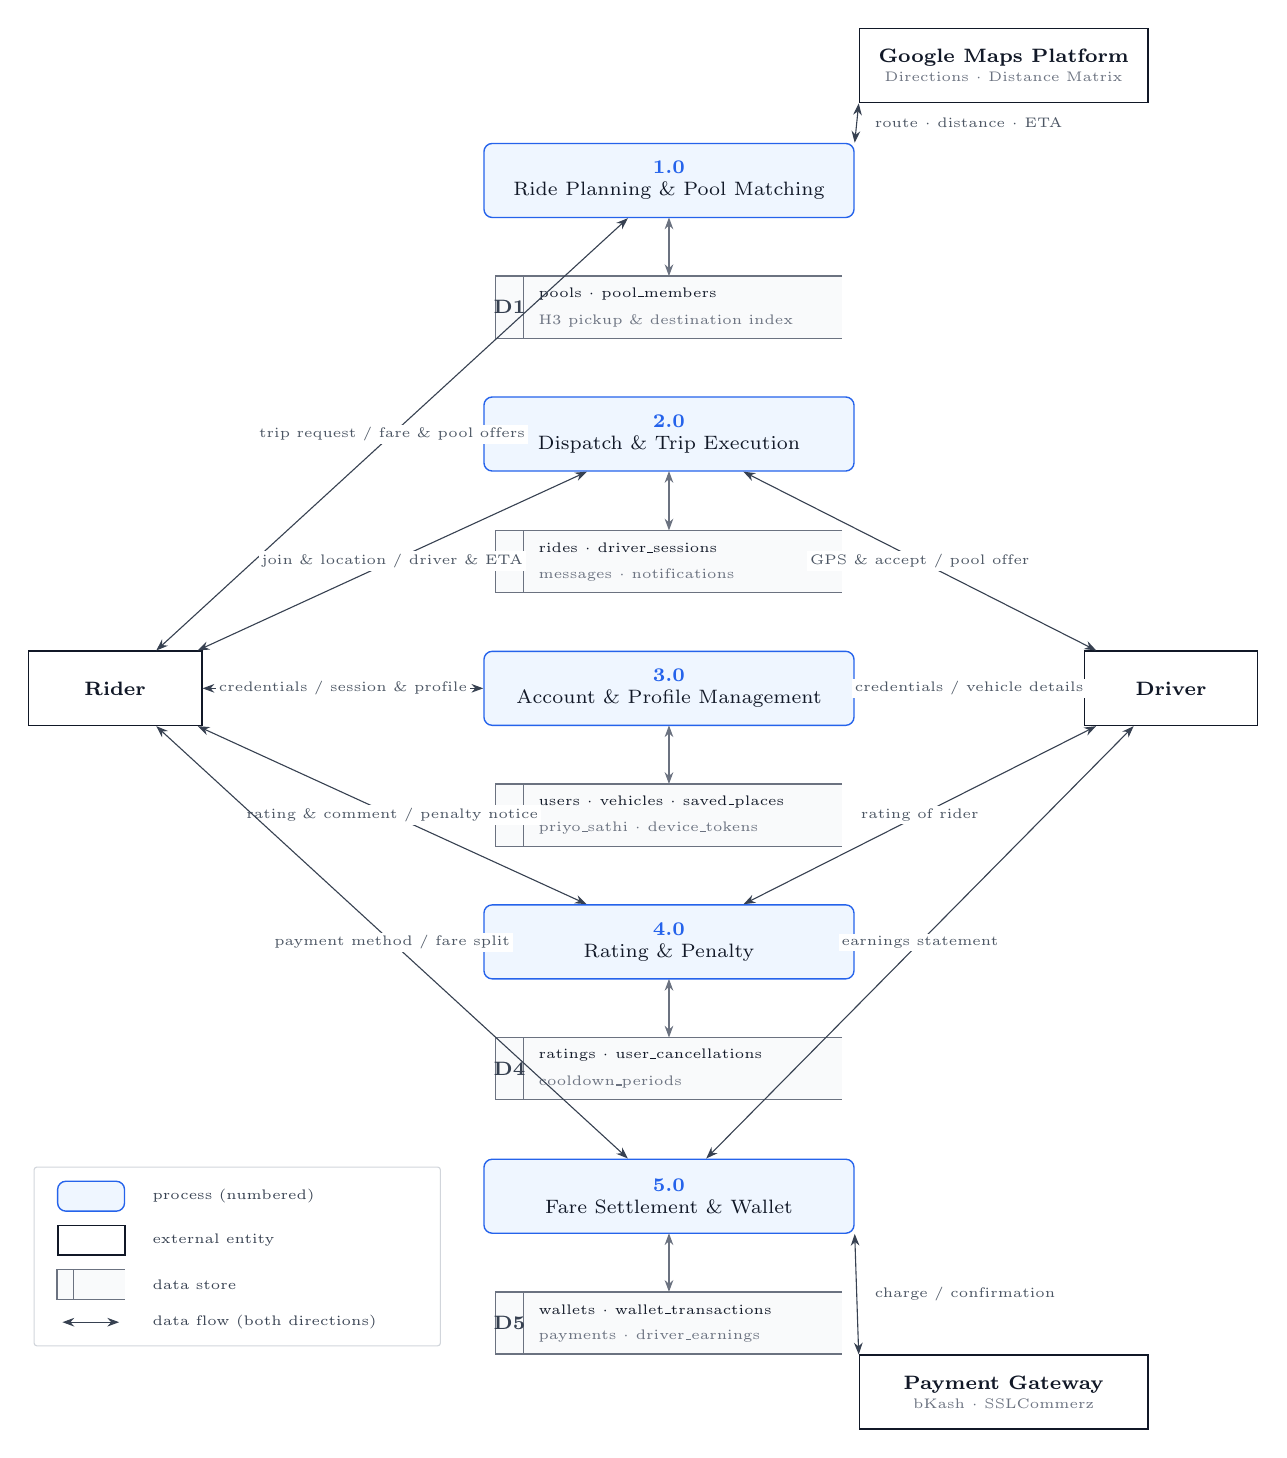
\begin{tikzpicture}

% ---------------- processes ----------------
\node[proc] (p1) at (8.793,16.12) {{\color{riderblue}\bfseries 1.0}\\Ride Planning \& Pool Matching};
\node[proc] (p2) at (8.793,12.90) {{\color{riderblue}\bfseries 2.0}\\Dispatch \& Trip Execution};
\node[proc] (p3) at (8.793, 9.67) {{\color{riderblue}\bfseries 3.0}\\Account \& Profile Management};
\node[proc] (p4) at (8.793, 6.45) {{\color{riderblue}\bfseries 4.0}\\Rating \& Penalty};
\node[proc] (p5) at (8.793, 3.22) {{\color{riderblue}\bfseries 5.0}\\Fare Settlement \& Wallet};

% ---------------- data stores ----------------
\dstore{8.793}{14.51}{D1}{pools $\cdot$ pool\_members}{H3 pickup \& destination index}
\dstore{8.793}{11.28}{D2}{rides $\cdot$ driver\_sessions}{messages $\cdot$ notifications}
\dstore{8.793}{ 8.06}{D3}{users $\cdot$ vehicles $\cdot$ saved\_places}{priyo\_sathi $\cdot$ device\_tokens}
\dstore{8.793}{ 4.84}{D4}{ratings $\cdot$ user\_cancellations}{cooldown\_periods}
\dstore{8.793}{ 1.61}{D5}{wallets $\cdot$ wallet\_transactions}{payments $\cdot$ driver\_earnings}

% ---------------- external entities ----------------
\node[ent]    (rider)   at ( 1.759, 9.67) {Rider};
\node[ent]    (driver)  at (15.168, 9.67) {Driver};
\node[extent] (gmaps)   at (13.043,17.58)
      {Google Maps Platform\\[-1pt]{\tiny\mdseries\color{midgrey}Directions $\cdot$ Distance Matrix}};
\node[extent] (gateway) at (13.043, 0.73)
      {Payment Gateway\\[-1pt]{\tiny\mdseries\color{midgrey}bKash $\cdot$ SSLCommerz}};

% ---------------- rider data flows ----------------
\draw[flow] (rider) -- (p1) node[lbl] {trip request / fare \& pool offers};
\draw[flow] (rider) -- (p2) node[lbl] {join \& location / driver \& ETA};
\draw[flow] (rider) -- (p3) node[lbl] {credentials / session \& profile};
\draw[flow] (rider) -- (p4) node[lbl] {rating \& comment / penalty notice};
\draw[flow] (rider) -- (p5) node[lbl] {payment method / fare split};

% ---------------- driver data flows ----------------
\draw[flow] (driver) -- (p2) node[lbl] {GPS \& accept / pool offer};
\draw[flow] (driver) -- (p3) node[lbl] {credentials / vehicle details};
\draw[flow] (driver) -- (p4) node[lbl] {rating of rider};
\draw[flow] (driver) -- (p5) node[lbl] {earnings statement};

% ---------------- external system data flows ----------------
\draw[flow] (gmaps.south west) -- (p1.north east)
      node[midway, anchor=west, xshift=3pt, font=\tiny, text=slategrey]
      {route $\cdot$ distance $\cdot$ ETA};
\draw[flow] (gateway.north west) -- (p5.south east)
      node[midway, anchor=west, xshift=3pt, font=\tiny, text=slategrey]
      {charge / confirmation};

% ---------------- process <-> data store ----------------
\draw[sflow] (8.793,15.65) -- (8.793,14.905);
\draw[sflow] (8.793,12.43) -- (8.793,11.675);
\draw[sflow] (8.793, 9.20) -- (8.793, 8.455);
\draw[sflow] (8.793, 5.98) -- (8.793, 5.235);
\draw[sflow] (8.793, 2.75) -- (8.793, 2.005);

% ---------------- legend ----------------
\begin{scope}[shift={(0.73,1.32)}]
  \draw[draw=hairline, line width=0.4pt, rounded corners=1pt] (0,0) rectangle (5.16,2.27);
  \node[proc, minimum width=0.85cm, minimum height=0.38cm, anchor=west] at (0.29,1.90) {};
  \node[anchor=west, font=\tiny, text=inkgrey] at (1.38,1.90) {process (numbered)};
  \node[ent, minimum width=0.85cm, minimum height=0.38cm, anchor=west] at (0.29,1.34) {};
  \node[anchor=west, font=\tiny, text=inkgrey] at (1.38,1.34) {external entity};
  \begin{scope}[shift={(0.72,0.78)}]
    \fill[surfacegrey] (-0.43,-0.19) rectangle (0.43,0.19);
    \draw[draw=midgrey, line width=0.5pt]
         (0.43,0.19) -- (-0.43,0.19) -- (-0.43,-0.19) -- (0.43,-0.19);
    \draw[draw=midgrey, line width=0.5pt] (-0.22,0.19) -- (-0.22,-0.19);
  \end{scope}
  \node[anchor=west, font=\tiny, text=inkgrey] at (1.38,0.78) {data store};
  \draw[flow] (0.36,0.30) -- (1.08,0.30);
  \node[anchor=west, font=\tiny, text=inkgrey] at (1.38,0.30) {data flow (both directions)};
\end{scope}

\end{tikzpicture}
% ============================= END FIGURE ============================
\end{document}
